\chapter{CARACTERIZAÇÃO DA ORGANIZAÇÃO}

A organização estudada é uma distribuidora de médio porte que atua no segmento de logística e distribuição atacadista. Seu serviço consiste em comprar mercadorias de fornecedores, recebê-las em um armazém próprio e entregá-las aos clientes --- mercados, padarias e restaurantes da região --- utilizando uma frota própria de vans e caminhões. Para o sistema, o tipo de produto vendido é irrelevante: tudo é tratado como \textbf{caixa}, isto é, um volume identificado por código de barras.

A empresa já possui um ERP, responsável pelo cadastro de clientes e fornecedores, pelos pedidos de venda e de compra, pela emissão de notas fiscais e pelo financeiro. Esse ERP, porém, não conhece caixas individuais, carregamentos, veículos nem motoristas, e só registra o pedido até o faturamento. A estrutura organizacional e as atribuições de cada área estão na Tabela~\ref{tab:areas}.

\begin{table}[htbp]
\centering
\caption{Estrutura organizacional da distribuidora}
\label{tab:areas}
\small
\begin{tabular}{|p{2.6cm}|p{4.4cm}|p{7.4cm}|}
\hline
\textbf{Área} & \textbf{Quem} & \textbf{Atribuição} \\ \hline
Comercial & Vendedores & Registram os pedidos dos clientes no ERP \\ \hline
Armazém & Conferentes e operadores & Recebem, guardam, separam e carregam caixas \\ \hline
Portaria & Porteiros & Controlam a entrada e a saída de veículos \\ \hline
Logística & Programador de cargas & Monta os carregamentos e escolhe veículo e motorista \\ \hline
Frota & Motoristas e responsável pela frota & Realizam as entregas e cuidam dos veículos \\ \hline
Gestão & Gerente & Acompanha a operação e resolve exceções \\ \hline
\end{tabular}
\fonte{Elaborado pelo autor (2026)}
\end{table}

Os principais processos formam um ciclo contínuo, ilustrado na Figura~\ref{fig:processo}: a entrada das caixas do fornecedor, o armazenamento, a montagem do carregamento a partir dos pedidos, a saída pela portaria, a entrega ao cliente e o retorno do veículo com as caixas não entregues.

\begin{figure}[htbp]
\centering
\caption{Processo operacional da distribuidora}
\label{fig:processo}
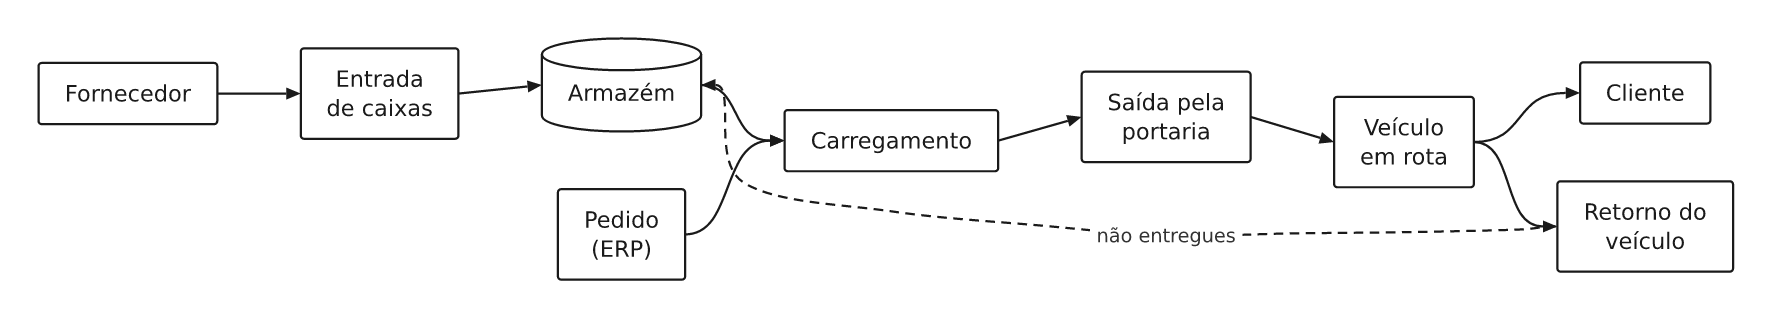
\includegraphics{figuras/processo.png}
\fonte{Elaborado pelo autor (2026)}
\end{figure}

Hoje, esses processos dependem de anotações manuais: o conferente conta as caixas olhando a nota e registra divergências em papel; o programador monta as viagens em planilha; o porteiro anota placas em um caderno; e o motorista avisa as entregas por mensagem. A Tabela~\ref{tab:problemas} resume os problemas identificados.

\begin{table}[htbp]
\centering
\caption{Problemas identificados no processo atual}
\label{tab:problemas}
\small
\begin{tabular}{|c|p{6.4cm}|p{7cm}|}
\hline
\textbf{\#} & \textbf{Situação atual} & \textbf{Consequência} \\ \hline
P1 & Entrada e saída anotadas em papel & Sem histórico confiável de quem, quando e o quê \\ \hline
P2 & Pedido sem acompanhamento após o faturamento & Cliente sem resposta e pedidos esquecidos \\ \hline
P3 & Carregamento em planilha e conferido no olho & Caixa no veículo errado ou deixada para trás \\ \hline
P4 & Portaria não confere a carga & Veículo sai com carga incompleta \\ \hline
P5 & Situação da frota em quadro na parede & Veículo em manutenção ou motorista com CNH vencida escalados \\ \hline
P6 & Retorno sem registro & Caixas extraviadas e pedidos que nunca terminam \\ \hline
\end{tabular}
\fonte{Elaborado pelo autor (2026)}
\end{table}

O problema central é, portanto, a \textbf{falta de rastreabilidade} das caixas e dos veículos. As oportunidades de melhoria por meio da tecnologia são claras: substituir anotações por leituras de código de barras no celular, aplicar automaticamente as regras de conferência e de liberação, e dar à gestão uma visão em tempo real da situação de cada pedido, caixa e veículo, sem substituir o ERP existente.
